\documentclass{standalone}

\usepackage{tikz}
\usepackage{amsmath}

% definition of all the colors
\usepackage{xcolor}
%New colors defined below
\definecolor{codecomment}{rgb}{0,0.6,0} % green
\definecolor{codegray}{rgb}{0.5,0.5,0.5} % gray
\definecolor{codestring}{rgb}{0.4,0.84,0.93} % blue
\definecolor{codebackgroundcolour}{rgb}{0.95,0.95,0.92}
\definecolor{corange}{RGB}{255, 70, 0} % orange
\definecolor{cyellow}{RGB}{209, 153, 0} % yellow
\definecolor{cblue}{RGB}{64, 128, 255} % blue
\definecolor{cbrown}{RGB}{153, 102, 51} % brown
\definecolor{cpink}{RGB}{255, 0, 255} % pink
\definecolor{cred}{RGB}{255, 64, 0} % red
\definecolor{cgreen}{RGB}{0, 191, 0} % green
\definecolor{clightblue}{RGB}{191, 217, 255} % light blue
\definecolor{clightgreen}{RGB}{224, 255, 224} % light green
\definecolor{clightpink}{RGB}{255, 230, 255} % light pink
\definecolor{cdarkblue}{RGB}{0, 0, 255} % dark blue

\begin{document}

%\tikzset{every picture/.style={line width=0.75pt}} %set default line width to 0.75pt        

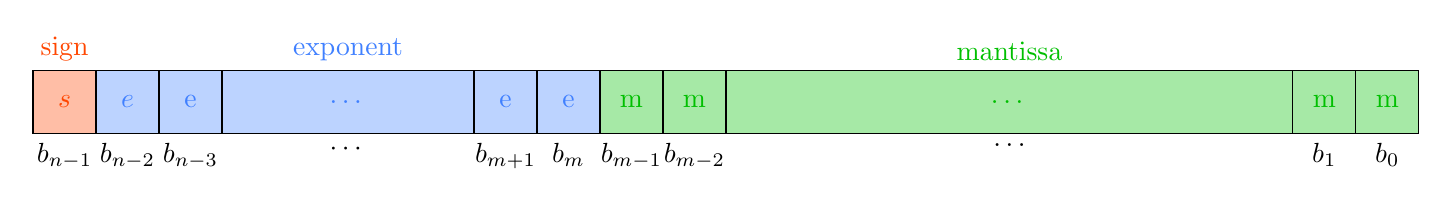
\begin{tikzpicture}


\coordinate (p);
\foreach \labela/\labelb/\inline/\c/\width in {
	\textcolor{corange}{sign}/$b_{n-1}$/$s$/corange/1,
	/$b_{n-2}$/$e$/cblue/1,
	/$b_{n-3}$/e/cblue/1,
	\textcolor{cblue}{exponent}/$\cdots$/$\dots$/cblue/4,
	/$b_{m+1}$/e/cblue/1,
	/$b_{m}$/e/cblue/1,
	/$b_{m-1}$/m/cgreen/1,
	/$b_{m-2}$/m/cgreen/1,
	\textcolor{cgreen}{mantissa}/$\ldots$/$\dots$/cgreen/9,
	/$b_1$/m/cgreen/1,
	/$b_0$/m/cgreen/1
}{
    \node[draw,fill=\c!35,minimum height=8 mm,minimum width=\width*8 mm,anchor=west,outer sep=0pt,label=below:\labelb,label=above:\labela]
    (n) at (p) {\textcolor{\c}{\inline}};
    %\draw[thick] ([yshift=-1mm]n.south west) -- ([yshift=1mm]n.north west);
    \coordinate (p) at (n.east);
}

\end{tikzpicture}


\end{document}